\chapter{Background}
\label{chap:background}

This work touches upon two topics in Computer Science: Semantic Web and Information Retrieval. The Semantic Web aims to add structure and semantics to the content of the Web. Information Retrieval focuses on providing users with answers to their queries. Our system is built upon user interfaces to provide users with suggestions of terms while building SPARQL queries. We thus conclude the chapter by discussing related works on the topic of User Interfaces for the Semantic Web.

% ##############################################################################################
% ##############################################################################################
% ##############################################################################################

\section{Semantic Web}

Every second, a humongous amount of data is added to the Web. This data comes in diverse flavours: photos, songs, movies, tweets, research papers, proprietary format files, blog posts, chats, database records, source code, weather data, you name it. It can also be in either the public domain like social media, news sites, knowledge bases; or in the private domain: corporate groups, closed forums, authorization required sites, etc. In either case, in order to access this information we depend on machines that crawl these sites and parse the information available using a variety of techniques: image classification, audio fingerprints, natural language processing, among others. In most cases, machines do not understand what the content is or how it is connected to other content. This leads to a number of shortcomings in how the content of the Web is managed, processed and used.

If you go to a Wikipedia article page about any topic, and then visit the same article page in a different language, it is quite likely that you will not find the same information in both pages. Factual information should not be different for different languages. As an example, let us consider \Cref{fig:eritreaWikipedia}. In both Spanish and English articles, Eritrea has a one million population difference. Likewise comparing other articles written in English and Spanish, the USA has 3 million and China has 4 million of a difference in population. While it may be argued that population is hard to measure, the Web is full of factual differences for the same subjects in different languages: in Wikipedia, users are in charge of manually editing documents and they might not use the same data across different languages, or data may not be updated so quickly in languages with fewer active editors.

\begin{figure}[!ht]
    \centering
        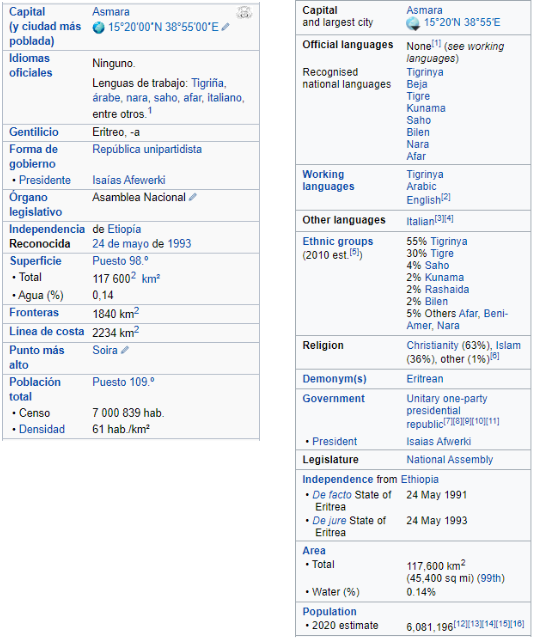
\includegraphics[width=.8\linewidth]{imagenes/EritreaWikipedia.png}
        \caption{Eritrea in both Wikipedia in Spanish and English.}
        \label{fig:eritreaWikipedia}
\end{figure}

Current research is opening many paths for parsing different types of data. In regards to text, a different approach is proposed by the W3C (World Wide Web Consortium). Instead of going from unstructured text to data, the Semantic Web proposes that data can be expressed on the Web in such way that both humans and machines can make use of it. In this proposal, the data is represented in a simple data model structure where common identifiers and standard vocabularies are used to connect the data across different Web domains. With this approach, pages (or parts of pages) could be generated from data and machines would have a better grasp of what the contents are. In the same way, information can be consolidated so that sites present the same information for different language versions.

This architecture proposal, known as the Semantic Web Stack is composed of different hierarchical language layers where higher layers are supported by lower ones (as in an OSI model or similar). As can be appreciated in \Cref{fig:semanticWebStack}, the stack is composed of several layers: a lower layer for identifiers and character set; a syntax layer; a data model layer; a query layer where also taxonomies, ontologies and rules are applied; a unifying logic layer; a proof layer; and a trust layer. All these layers together support user interfaces and applications. A transversal cryptography layer is proposed to support identity verification and encryption of sensitive data. It is important to mention that the stack is under evolution: there are several research proposals for changes to its structure. We will focus on the main layers in this section.

\begin{figure}[H]
    \centering
        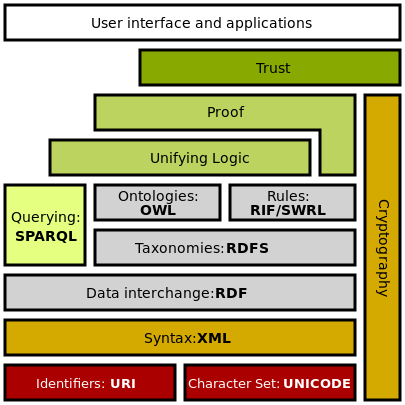
\includegraphics[width=.5\linewidth]{imagenes/Semantic_web_stack.png}
        \caption{Semantic Web Stack \cite{SemanticWebWikipedia}}
        \label{fig:semanticWebStack}
\end{figure}

The lowest layer defines character encoding and identifiers. The Unicode standard is used for character encoding and IRIs (Internationalized Resource Identifier\footnote{An IRI is a generalization of an Unified Resource Identifier (URI) on Unicode.}) for identifiers. This two-part layer supports unambiguous identification of each resource using characters and symbols from different alphabets.

Above this layer sits the syntax layer. This layer defines the grammar and how the identifiers are structured. While XML is the defined standard, N-Triples~\cite{nTriples} and Turtle~\cite{Turtle}  are the most commonly used for syntax and structure. According to their own definitions, "N-Triples is a line-based, plain text format for encoding an RDF graph."~\cite{nTriples} and "Turtle allows RDF statements to be completely written in a compact and natural text form, with abbreviations for common usage patterns and datatypes"~\cite{Turtle}. We can see an example of RDF data in Turtle format in \Cref{fig:turtleExample}. 

\begin{figure}[H]
\begin{minted}[]{sparql}
@prefix ex:    <http://example.org/> .

ex:Earth ex:highestPoint ex:MountEverest .
ex:Asia ex:partOf ex:Earth .
ex:Asia ex:sharesBorderWith ex:Europe .
ex:Europe ex:partOf ex:Earth .
ex:MountEverest ex:continent ex:Asia .
ex:MountEverest ex:namedAfter ex:GeorgeEverest .
ex:GeorgeEverest ex:countryOfCitizenship ex:UnitedKingdom .
ex:GeorgeEverest ex:placeOfDeath ex:London .
ex:UnitedKingdom ex:continent ex:Europe .
ex:UnitedKingdom ex:capital ex:London .
\end{minted}
\caption{Example of RDF data in the Turtle format}
\label{fig:turtleExample}
\end{figure}

In our example, prefixes stay on top of our file and define abbreviations for our data. On the bottom are our subject-predicate-object triples. The same example could be written in N-Triples format.\footnote{To see how these formats compare, the EasyRdf web service: \url{http://www.easyrdf.org/converter} allows users to translate data formats in a simple way.} 

Following the Syntax layer are the data interchange or data model layer and the query layer. We will discuss more about these in \Cref{chap:RDF} and \Cref{chap:SPARQL}. The taxonomies, ontologies and rules layer define how the data fits together: relations and vocabularies are defined in these layers.

On top of these layers we can find the unifying logic, proof and trust logic. While these layers are not completely theoretically defined, they are defined as a proof-of-concept. The unifying logic layer combines ontological reasoning with querying. The proof layer provides a proof of procedures or information to the client, and the trust layer defines access control between services and data.

Regarding the Semantic Web, the state of the art is constantly expanding with new research methods to improve reach, performance or usability in order to bring the Semantic Web closer and closer to users. Some well-known fields where Semantic Web has had notable contributions are drug discovery, patient care management and reporting, publication of scientific knowledge, drug approval procedures, music and movie databases, geospatial data, etc. Interesting works for the author are applications in the industrial sector, for instance where process data from IoT or RFID sensor data is added every second to RDF datastores \cite{Zhang2018,Soylu2018,Kharlamov2016}. In the author's national context, the Chilean Library of Congress has its data available in RDF format~\cite{datosbcn}.

% ##############################################################################################
% ##############################################################################################
% ##############################################################################################


\subsection{Data Model RDF}
\label{chap:RDF}

The Resource Description Framework (RDF) \cite{rdfConcepts, rdfprimer11} is at the core of the Semantic Web. RDF proposes a data interchange model for structuring factual content for interoperability between different data sources (usually the Web, but it can be applied to anything). The goal of the standard is to "facilitate data merging even if the underlying schemas differ, and it specifically supports the evolution of schemas over time without requiring all the data consumers to be changed."~\cite{W3CRDF}. The standard defines RDF terms, triples, graphs and vocabularies. RDF is currently on version 1.1, published in 2014.

An RDF term represents a resource. A resource can either be an IRI, a literal value or a blank node. An IRI is an unambiguous identifier for a resource. Literal values can be text strings or datatypes (integer, boolean, double, datetime, etc.). Literal text strings can be defined in an specific language by adding a language tag: i.e.: "@en" represents a literal text string in English. A blank node (or \textit{bnode}) is used to represent a resource whose identifier or literal is not given. Blank nodes can be seen as denoting anonymous resources.

RDF triples or simply \textit{triples} allow the construction of a statement that relates RDF terms. Three RDF terms can be grouped to create a 3-tuple subject-predicate-object statement: "Mary eats pizza". This format allows for both humans and machines to easily read, query and reason about a data statement. 
In this 3-tuple, the subject identifies which resources the statement is about; the predicate indicates the relationship, traits or aspects between the subject and the object; the object identifies the value of the statement. From this basic 3-tuple structure and using blank nodes, statements can grow in complexity: for example, we can represent the statement "Mary eats (pizza madeOf mozzarella)" using a blank node to represent the pizza.

RDF defines certain grammar rules or semantics \cite{RDFSemantics} for building triple statements:
\begin{itemize}
    \item Subjects must be an IRI or blank node.
    \item Predicates must be an IRI.
    \item Objects can be either an IRI, literal or a blank node.
\end{itemize}

A collection of triples represents a labeled directed multi-graph or simply an RDF \textit{graph}. In RDF graphs, subjects and objects represent nodes and predicates represent labels on directed edges connecting them. In \Cref{fig:bobMarleyExampleGraph} we can appreciate how our RDF data from \Cref{fig:turtleExample} visually looks like.

\begin{figure}[h!]
    \centering
        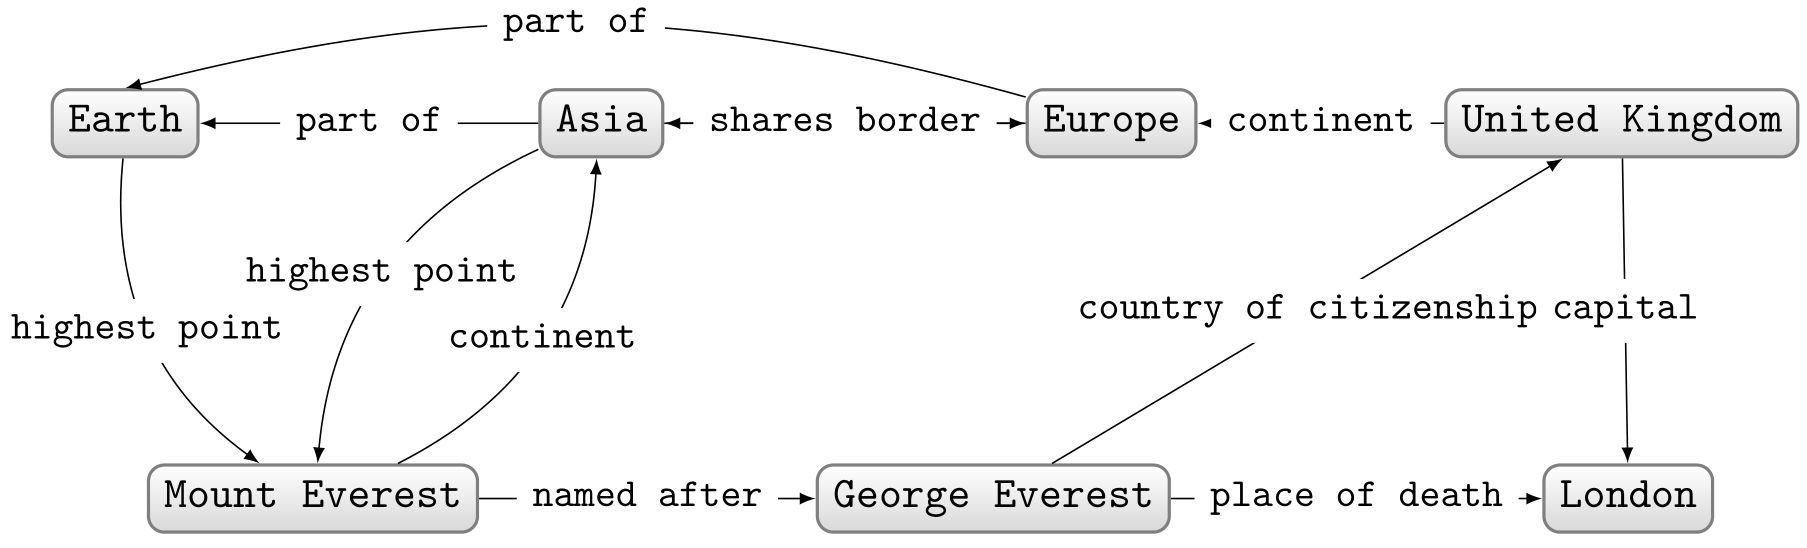
\includegraphics[width=.9\linewidth]{imagenes/exampleGrapha.png}
        \caption{Graph representation of our \Cref{fig:turtleExample} example data~\cite{Moreno2018}}
        \label{fig:bobMarleyExampleGraph}
\end{figure}

RDF vocabularies are built on top of the RDF standard. They add meaning to the relationships within our data. Classes (aka types) and properties (aka relationships) are defined for resources. Classes support class hierarchies, grouping, organization and processing of resources. For example, we may define the classes \textit{City} and \textit{Country} and define them to be subclasses of the more general class \textit{Place}. Properties are extended by the use of vocabularies: ontologies, taxonomies and thesauri are defined to simplify data sharing across diverse applications and enable richer integration and interoperability of data among descriptive communities. Properties may also form a hierarchy, and may have domain and ranges classes to indicate the types of the subjects and objects that they relate. For example, we may define a property \textit{hasCapital} as a subproperty of \textit{hasCity}, both of which have the domain \textit{Country} and range \textit{City}.

Vocabularies are defined in their own standards: RDF Schema (RDFS)~\cite{RDFS}, Web Ontology Language (OWL)~\cite{OWL} and Simple Knowledge Organization System (SKOS)~\cite{SKOS} are powerful technologies to structure and organize data. As per their own reference sites: "RDFS is a general-purpose language for representing simple RDF vocabularies on the Web"~\cite{RDFS}. "OWL is a computational logic-based language such that knowledge expressed in OWL can be exploited by computer programs, e.g., to verify the consistency of that knowledge or to make implicit knowledge explicit"~\cite{OWL}. "SKOS is a common data model for sharing and linking knowledge organization systems via the Web"~\cite{SKOS}. From these vocabularies, we use the following properties in this work: \textit{label}, \textit{alternative label} and \textit{description}. We will not use ontologies and reasoning in this current work, and thus we will not dive deeper into these topics.

% ##############################################################################################
% ##############################################################################################
% ##############################################################################################

\subsection{SPARQL}
\label{chap:SPARQL}

In the previous section we went through the data model to store Semantic Web data. In this section we will focus on how to retrieve this data. SPARQL~\cite{SPARQL} is the W3C standard for querying RDF data. As per the SPARQL reference site: "SPARQL can be used to express queries across diverse data sources, whether the data is stored natively as RDF or viewed as RDF via middle-ware. SPARQL contains capabilities for querying required and optional graph patterns along with their conjunctions and disjunctions. SPARQL also supports extensible value testing and constraining queries by source RDF graph. The results of SPARQL queries can be results sets or RDF graphs."~\cite{SPARQL}

SPARQL uses a syntax similar to SQL (Structured Query Language) for RDF triples. SPARQL query statements are expressed in the RDF Turtle syntax extended with SPARQL keywords. In these statements, clauses are expressed. A clause can contain triple patterns, in which elements of the triple (subject-predicate-object) can be replaced by variables in order to query for specific data.

In our following example, based on our \Cref{fig:turtleExample} example data, we present a simple query on how to get the highest mountain on Earth and in which continent it is located. This query will return the pair \texttt{ex:MountEverest}, \texttt{ex:Asia} because \texttt{?highest} matches in the \texttt{WHERE} clause with \texttt{ex:MountEverest} in the dataset and the same with \texttt{?continent} matching \texttt{ex:Asia}.

\begin{figure}[H]
\begin{minted}[]{sparql}
SELECT ?highest ?continent
WHERE {
    ex:Earth ex:highestPoint ?highest .
    ?highest ex:continent ?continent
}
\end{minted}
\caption{Example of a SPARQL query.}
\label{fig:sparqlQueryExample}
\end{figure}


% ##############################################################################################
% ##############################################################################################
% ##############################################################################################

\subsection{Linked Data}

While the Semantic Web refers to the standards used for storing, relating and querying our human/machine-friendly data, Linked Data is the term used for best practices or principles applied to this data. These principles, according to the reference site~\cite{LinkedData} are as follows:

\begin{itemize}
    \item Use URIs as names for things
    \item Use HTTP URIs so that people can look up those names.
    \item When someone looks up a URI, provide useful information.
    \item Include links to other URIs so that they can discover more things.
\end{itemize}

Using these principles, our goal is to use the Semantic Web standards to represent and access data on the Web, while being able to link (thus the name Linked Data) different resources. The idea is to be able to connect all resources into a global data graph on the Web that users can easily navigate and refer to.

The Linked Data principles have been growing in adoption since their proposal, with multiple community and private RDF datasets available. Many of these Linked Data sites provide clients with user interfaces, APIs and query endpoints for accessing the data using SPARQL or direct navigation. 

A compilation of publicly available linked data sites can be found on \url{https://lod-cloud.net}. Currently the site contains 1,255 datasets with 16,174 links between them (As of May 2020). Datasets in this site are classified in the following categories: Cross-Domain, Geography, Government, Life Sciences, Linguistics, Media, Publications, Social Networking and User-Generated. In this work, we are going to use the Wikidata dataset as our proof of concept~\cite{wikidataQueryService}, but our methods extend likewise to other datasets. We will talk more about this dataset in the following section.

% ##############################################################################################
% ##############################################################################################
% ##############################################################################################

\subsection{Wikidata}

In this work we are going to use RDF data from the \url{https://www.wikidata.org/} site for evaluating our proposal. Wikidata is a free, collaborative, multilingual and open knowledge base that can be read and edited by both humans and machines~\cite{Wikidata2014}. Wikidata acts as central storage for collecting structured data to provide support for Wikipedia, Wikimedia Commons, the other wikis of the Wikimedia movement, and to anyone in the world.

To date, Wikidata describes over 84 million resources with over 5,126 million statements\footnote{\url{https://www.wikidata.org/wiki/Wikidata:Statistics}}. Wikidata resources are uniquely identified by a letter \textit{Q} followed by a number, such as \textit{Douglas Adams (Q42)}. Statements describe detailed characteristics of a resource and consist of a property and a value. Properties in Wikidata have a letter \textit{P} followed by a number, such as with \textit{educated at (P69)}. For Douglas Adams' example, he was educated at the \textit{St. John's College (Q691283)}. The previous example, taken from the Wikidata introduction site, also provides \Cref{fig:wikidataDataModel} to show how this RDF data could be presented to users.

\begin{figure}[h]
    \centering
        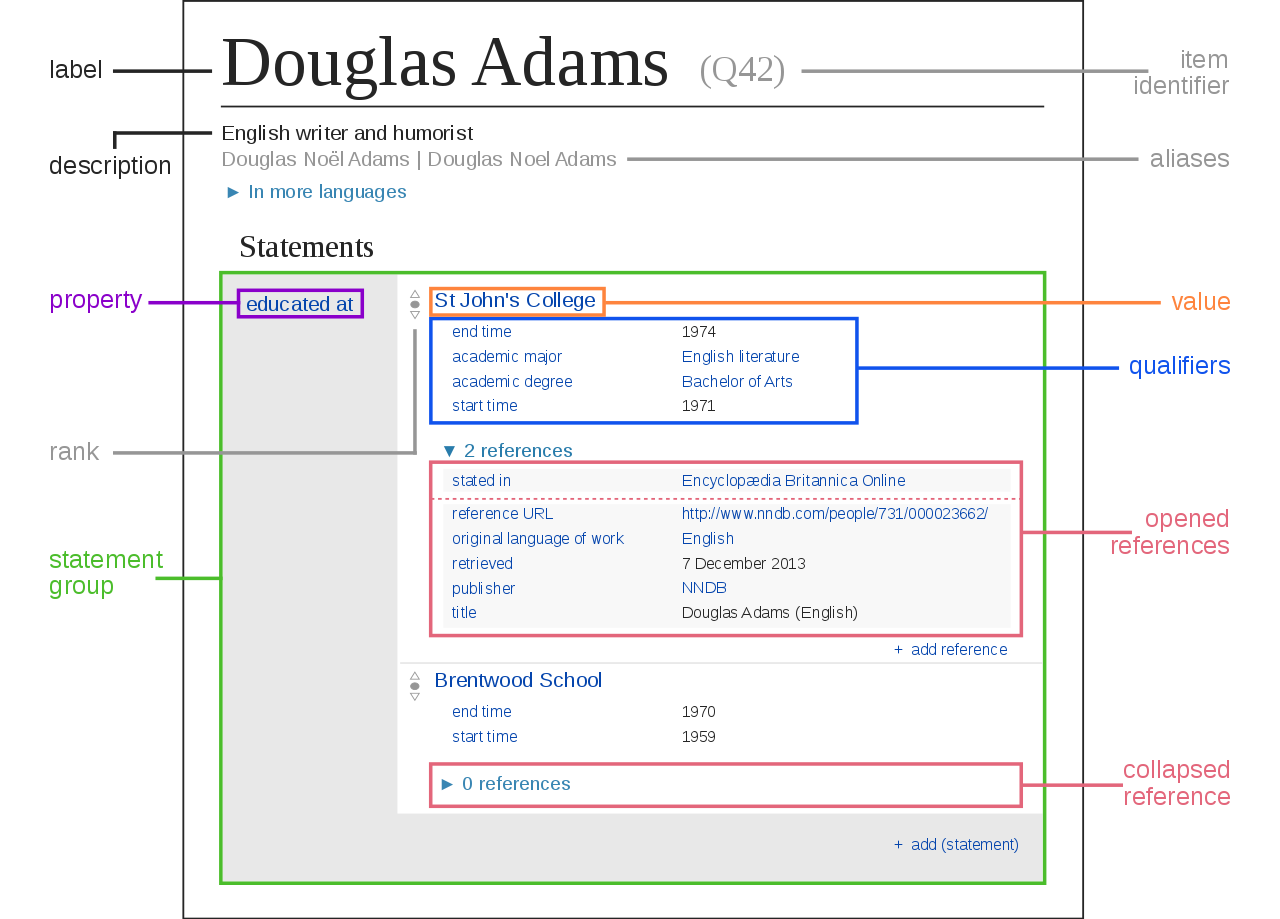
\includegraphics[width=\linewidth]{imagenes/Datamodel_in_Wikidata.png}
        \caption{Wikidata Model. From the Wikidata introduction site~\cite{WikidataIntroduction}}
        \label{fig:wikidataDataModel}
\end{figure}

It is possible to download a copy of the whole Wikidata knowledge base in RDF/N-Triples format. This 41 GBytes compressed RDF dump contains the previously mentioned information as RDF triples. The RDF triples that model the previous example are presented in \Cref{fig:rdfDataExample}. This data is publicly available at the \url{https://dumps.wikimedia.org/wikidatawiki/entities/} site. While it is possible to instantiate different SPARQL engines to query this database~\cite{Hernandez2016}, we will be working with the plain N-Triples data dump. For querying purposes, we will use the Wikidata API available at \url{https://www.wikidata.org/w/api.php}.

\begin{figure}[H]
\begin{minted}[]{sparql}
# Single line comments begin with the '#' character
# Label
wd:Q42 rdfs:label "Douglas Adams"@en . 
# Alternative labels
wd:Q42 skos:altLabel "Douglas N. Adams"@en .
wd:Q42 skos:altLabel "Douglas Noel Adams"@en .
# Description
wd:Q42 schema:description "English writer and humorist"@en .
# Properties, such as place of birth (P19), country of citizenship (P27), 
# instance of (P31), educated at (P69) and residence (P551).
# The next line reads: Douglas Adams' place of birth is Cambridge (Q350).
wd:Q42 wdt:P19 wd:Q350 .
wd:Q42 wdt:P27 wd:Q145 .
wd:Q42 wdt:P31 wd:Q5 .
wd:Q42 wdt:P69 wd:Q691283 .
wd:Q42 wdt:P551 wd:Q84 .
\end{minted}
\caption{Example RDF data for Douglas Adams in Wikidata (Q42).}
\label{fig:rdfDataExample}
\end{figure}

% ##############################################################################################
% ##############################################################################################
% ##############################################################################################

\section{Information Retrieval}

In the previous section we introduced some key Semantic Web concepts. While these concepts will be relevant in terms of the type of information that we process, we require techniques from another field of Computer Science to  be able to process and manage this information. The field called Information Retrieval is concerned with finding information from large collections. In order to find this information, this field uses indexes and relevance measures to store and classify the information. For our work, we will be using Inverted Indexes to store and search information, while using Term-Frequency-Inverse-Document-Frequency (TF-IDF) and PageRank for ranking the results.

\subsection{Inverted Index}
\label{chap:lucene}

In our research we take information about Semantic Web resources described using RDF and store it in an specialized index. In this index, we will store information about RDF resources, such as the identifier (subject id), the label, description, alternative labels, outgoing properties (predicates available) and so on. This information is extracted from the triples associated with a resource. We will go into more detail on this in \Cref{chap:index}.

Since much of the information that we are going to index is text based, a suitable index is an inverted index. In a forward index, like relational databases, each resource is stored by its id and all available fields are accessed through that id. In an inverted index, fields are stored and the resource ids are accessed by searching over the fields. Inverted indexes are commonly used for text document indexing, where a collection of words are indexed. Every time a user searches for something, they will query these words and the documents containing them will be returned as results.

In this work we will build a document for every resource described by the RDF graph, where our label, alternative labels and descriptions will work as our different text fields. With this index, we will be able to search for words, such as "\textit{capital of Seychelles}" and as an answer we would get all documents that contain these words. Among the results we will get \textit{Victoria} and also \textit{Seychelles} (while also getting other capital-related documents). In order to get this to work properly, our index will deal with different kinds of fields:

\begin{itemize}
    \item Text fields contain text and ignore stop words and group similar words.
    \item Numeric fields allow us to store integers or doubles, while providing support for sorting and range queries.
    \item String fields look for exact matches, such as the name of our resource subject name.
    \item Stored fields allow us to save information that is not required for querying, such as our predicates.
\end{itemize}

There are two more points worth mentioning for inverted indexes. Since we are processing some of the input data while building our index, inverted indexes take longer to create than forward indexes. The other point is relevance: Inverted indexes can sort the queried results by certain criteria: 

\begin{itemize}
    \item Matching a word in the label of a document might be more relevant than matching a word in the description of it.
    \item Rare words that might appear less frequently in the collection of documents boost the relevance of our results.
    \item Matching several words in our query pattern might also bump the relevance of our results up.
    \item Words occurring more frequently in a document indicate higher relevance.
\end{itemize}

A ranking measure based on these criteria is known as TF-IDF and is one of the ranking measures that we will implement for our text-based lookups. In the following section, we will cover how TF-IDF is not the only measure that we will implement and we will also cover why another measure is helpful.

% ##############################################################################################
% ##############################################################################################
% ##############################################################################################

\subsection{Ranking}
\label{chap:pagerank}

In the previous section we mentioned which indexing method we will use and how it inherently implements a ranking measurement for sorting query results. We mentioned that, while this TF-IDF is in place, another ranking measure may help our users to get better results.

Let us take for example "Jordan". On the one hand we have the country, while on the other we have the basketball player. If you go to Google and search for Jordan, what would you expect to be shown first? This is a hard question to answer. In order to estimate the resources relevant to a keyword search that a user is most likely to be interested in, an importance metric algorithm is implemented next to our relevance ranking metric: based on how many references links-to and how many other resources are linked-from a resource, an importance ranking value can be set to better optimize results.

A similar approach for link-based ranking, proposed in 1998 by Google's founders Larry Page and Sergey Brin, is known as PageRank~\cite{Page1998}. It was first conceived to add importance ranking to web sites. In their proposal, web sites are modelled as a directed graph: Each web site is a node, web sites may have incoming links (links that direct to that site) and outgoing links (links that direct to other sites). After modelling the web like this, a recursive algorithm takes place: A page with lots of inlinks from important pages with few outlinks is more important. There are some scenarios to consider: when a document has no links and when two documents link only to each another. In order to avoid high relevance from these cases, there is a probability to not follow any link and jump to a random document.

The PageRank process sets an initial value to all documents: this value is the same for all, such that the sum of all document’s rank is 1. The next step will be to share the document's rank to all documents it links to: a higher ranked document gives a higher rank to its links, while documents with lots of links give a low rank because its rank is divided across all its links. With the probability to jump randomly (usually set as 0.15), this process is recursive and guarantees to converge, so after a number of iterations each document’s rank is fixed.

For our research, we are not dealing with web sites but with RDF resources that link to other RDF resources, thus this application also fits our needs. PageRank will work by considering the incoming and outgoing edges between RDF resources (see \Cref{fig:bobMarleyExampleGraph}) as the incoming and outgoing links in web sites. Using both our PageRank importance and the TF-IDF relevance, query results are sorted and returned to our users. This approach can be used to rank the nodes of an RDF graph, namely the terms appearing as the subject and/or object of one or more triples. However, PageRank is not directly applicable to rank property terms. In order to rank properties, we rather use the frequency of the property in terms of how many triples in the RDF graph use that property. We assume that users will often be interested in properties that are most frequently defined in the data.

% ##############################################################################################
% ##############################################################################################
% ##############################################################################################

\section{User Interfaces}

In \Cref{chap:SPARQL} we covered SPARQL, the W3C standard for creating RDF queries. While this approach serves the purpose of creating queries, it requires an understanding of both the SPARQL language syntax and the underlying RDF data structure: which properties exist and how they interrelate resources. As we mentioned before, other authors have identified that these are two main issues limiting Semantic Web adoption by non-technical users: SPARQL language syntax and the lack of helpful user interfaces~\cite{Ferre2016, Lehmann2014, Unger2014}.

The third field of Computer Science that will take part in our research will be User Interfaces. How will our users engage with our system? How will we support their journey of using Linked Data? There are two pieces that fit our work: We will use visualization and query interfaces to help users explore, navigate and create SPARQL queries in an interactive way (without dealing with SPARQL); and we will use autocomplete to support the selection of results from a collection of candidate suggestions. 

Autocomplete or picklists allow users to narrow a collection of results by typing characters that get the users closer to their desired result. There are several techniques that can be implemented under an autocomplete user control. Fuzzy search or approximate string matching is a technique to find strings that match a pattern approximately, rather than exactly. Debounce timers allow autocomplete user controls to wait some time before submitting a query: this makes the system more fluent, skipping immediate changes (like adding/removing single characters) and waiting for users to elaborate on their query terms before firing another search event.

In other application fields, autocomplete can be easily be implemented since the scope is relatively fixed or small. In relational databases the structure or schema of the database is fixed independent of the size of the database. While the schema can change, its modifications are not as dynamic as the data itself. In IDEs on the other hand, the source code structure is dynamic, but the size of this structure is not a problem for a modern IDE and changes are handled on the go. This autocomplete indexing process can be experienced when importing a large codebase into a modern IDE. The system will require several minutes before any suggestions can be provided. In contrast with relational databases, RDF graphs do not have something analogous to a relational schema, likewise the scale of RDF graphs is often greater than the scale of a codebase.

Visualization and query interfaces aim to help users navigate, explore and build queries without necessarily writing code by means of displaying resources and connecting them in an easy-to-use visual user interface. These systems also support users in navigation tasks, by displaying information of a subject and its relation with others. Most such systems are designed for a specific language. While there are multiple recommendations and studies related to these types of user interfaces~\cite{Dadzie2011, Bikakis2016}, there are no defined rules or standards that guide the development of these systems. In the following section we will cover some of the existing research work available for these topics in the context of RDF data.

With regards to visualization and exploration of RDF data, we have studied two surveys that cover this topic. Dadzie et al.'s work: "Approaches to visualising Linked Data: A survey"~\cite{Dadzie2011}, studies several existing systems, classifies and evaluates them according to their scalability, as well as their features for filtering, data overview, text/graph view, faceted search, among others. Their statement is that for users to better understand the underlying structure of RDF triplestores, a key solution "is to visualise Linked Data in a coherent and legible manner, allowing non-domain and non-technical audiences to obtain a good understanding of its structure, and therefore implicitly compose queries, identify links between resources and intuitively discover new pieces of information."

A follow-up survey conducted in 2016 by Bikakis et al.: "Exploration and Visualization in the Web of Big Linked Data: A Survey of the State of the Art"~\cite{Bikakis2016} makes a sweep through the state of the art systems for exploration and visualization. 
Their work states how "exploring and visualization of very large dataset has become a major research challenge, of which scalability is a vital requirement". They also describe some major prerequisites and challenges that should be addressed by modern exploration and visualization tools.
In their research, they identify that most traditional exploration and visualization tools operate in an offline way, limited to small datasets, and not being able to explore large-scale datasets, such as the one that we will be using in this work.

Regarding autocomplete, some authors have approached the idea of adding autocomplete support to SPARQL queries. 
In their research work "Designing scientific SPARQL queries using autocompletion by snippets" Rafes et al.~\cite{Rafes2018} have conducted a two year study on SPARQL queries expressed by a community of scientific users. 
In this work they have studied different text query editors\footnote{Flint Editor, iSPARQL, LODatio+, BioCarian, Gosparqled, Wikidata Query and YASGUI. All cited by Rafes et al.~\cite{Rafes2018}} with autocomplete features and classified them into four main techniques: 
\textit{Autocompletion using relative IRIs via keywords}; 
\textit{Autocompletion by prefix declaration}; 
\textit{Autocompletion by template}; and 
\textit{Autocompletion by suggestion of snippets}. 
They have also identified that users usually fail to express SPARQL queries due "to imperfect knowledge on the ontologies involved in the queries or the need to follow a syntax rather complex to master"~\cite{Rafes2018}. 
Their work is based on "suggesting fragments of queries made by other previous users to complete the partial query already written by the user"~\cite{Rafes2018}.
It works by "extracting representations of subpatterns from previous queries (in the form of 'linegraphs') and construct a hierarchical clustering of such subpatterns to generate snippets that are most compatible with the portion of the query considered by the user"~\cite{Rafes2018}. Our methods are similar in that we provide suggestions to users, but based on the data that exists in the triplestore itself.

Another approach to autocompletion has been proposed by El-Roby et al.~\cite{El-Roby2016}. 
In their work "Sapphire: Querying RDF Data Made Simple", they propose "a tool that helps users write syntactically and semantically correct SPARQL queries without prior knowledge of the queried datasets."~\cite{El-Roby2016}
In their study, they have identified that Natural Language approaches for querying are good for simple queries, but not for complex queries. 
For complex queries, they remark that "the user needs to know the structure of the dataset, the vocabulary used to represent different concepts, and the literals used in the dataset including their data types and format."~\cite{El-Roby2016}
Their system "provides data-driven suggestions to complete the predicates and literals in the query"~\cite{El-Roby2016}. 
As in our work, their architecture is based on a server that sits between the user and the SPARQL endpoint.
The indexing mechanics between Sapphire and our work differ mainly on two points: 
They build their index with a sample of the data, built by running multiple queries (17 hours of queries for DBpedia), on the remote endpoint for hierarchical relations and predicates; 
the second difference is that their proposals are based on properties that point to literals and not entity-to-entity relations.

There are a couple of visual query/exploration systems that we found interesting in the context of this work: "VIQUEN: A visual query engine for RDF" by Dell~\cite{Dell2010}, "Node-centric RDF Graph visualization" by Sayers~\cite{Sayers2004}, "ViziQuer: a Web-based tool for visual diagrammatic queries over RDF data" by Cerans et al.~\cite{Cerans2018}, "FedViz: A Visual Interface for SPARQL Queries Formulation and Execution" by ~\cite{Zainab2015}, among others. From studying these works, we have noted that some rely either on domain specific, offline local triplestores, SPARQL-syntax-based queries or direct-to-endpoint queries for data retrieval. These works set important precedents for exploration and navigation of triplestores.

The visual query system "Smeagol: A 'Specific-to-General' Semantic Web Query Interface Paradigm for Novices" by Clemmer et al.~\cite{Clemmer2011} helps users to build queries that "guides the user from a specific example to a general result set". This novel approach is very helpful since it allows users to navigate and explore the data until they build a concrete subgraph of interest which then can be generalized to find other subgraphs similar to the one identified. Their work provides some interesting features such as autocompletion, dynamic results (query results are generated and used during query construction, which in turn helps building a better query), and non-emptiness guarantees. We find two drawbacks on their work: their system is only able to build tree-shaped queries and does not support general graph patterns; and their exploration tasks are done directly over the remote SPARQL endpoint, which faces the problems described before.

Vargas et al. in their "RDFExplorer: A Visual SPARQL Query Builder" research take Smeagol as a base system to develop further. Their work, as we mentioned before, supports users in navigation and query building tasks while displaying dynamic results during query building. We have found their interface to be very easy to use and supports keyword lookups for entities and properties with autocomplete features. An improvement upon Clemmer's work is that this research supports multiple graph patterns with cycles. Still, the system gets the suggestions by querying the endpoint directly, which can end in timeouts for many user queries. An additional advantage of this research, is that the source code is publicly available at \url{https://github.com/hvarg/RDFExplorer} while also having a live version available at \url{https://www.rdfexplorer.org/}.